\subsection{Le calorimètre hadronique ou HCAL}\label{chapter-LHC-section-CMS-subsec-HCAL}
%\cite{cms_paper,CERN-LHCC-97-031,CMS-DP-2016-071,CMS-DP-2017-016,CMS-DP-2017-017,CMS-DP-2017-033,CMS-DP-2017-034,CMS-DP-2017-042,CMS-DP-2018-018,CMS-DP-2018-019}
Le calorimètre hadronique (HCAL)~\cite{cms_paper,CERN-LHCC-97-031,CMS-TDR-10} permet de mesurer l'énergie des hadrons par un processus destructif.
Le HCAL étant situé à l'intérieur du solénoïde de CMS, les particules y déposant leur énergie ne sont donc pas perturbées par une traversée du solénoïde.
La figure~\ref{fig-chapter-LHC-section-CMS-subsec-HCAL-cms_paper-fig_5-1} représente l'agencement du HCAL.
\begin{figure}[b]
\centering
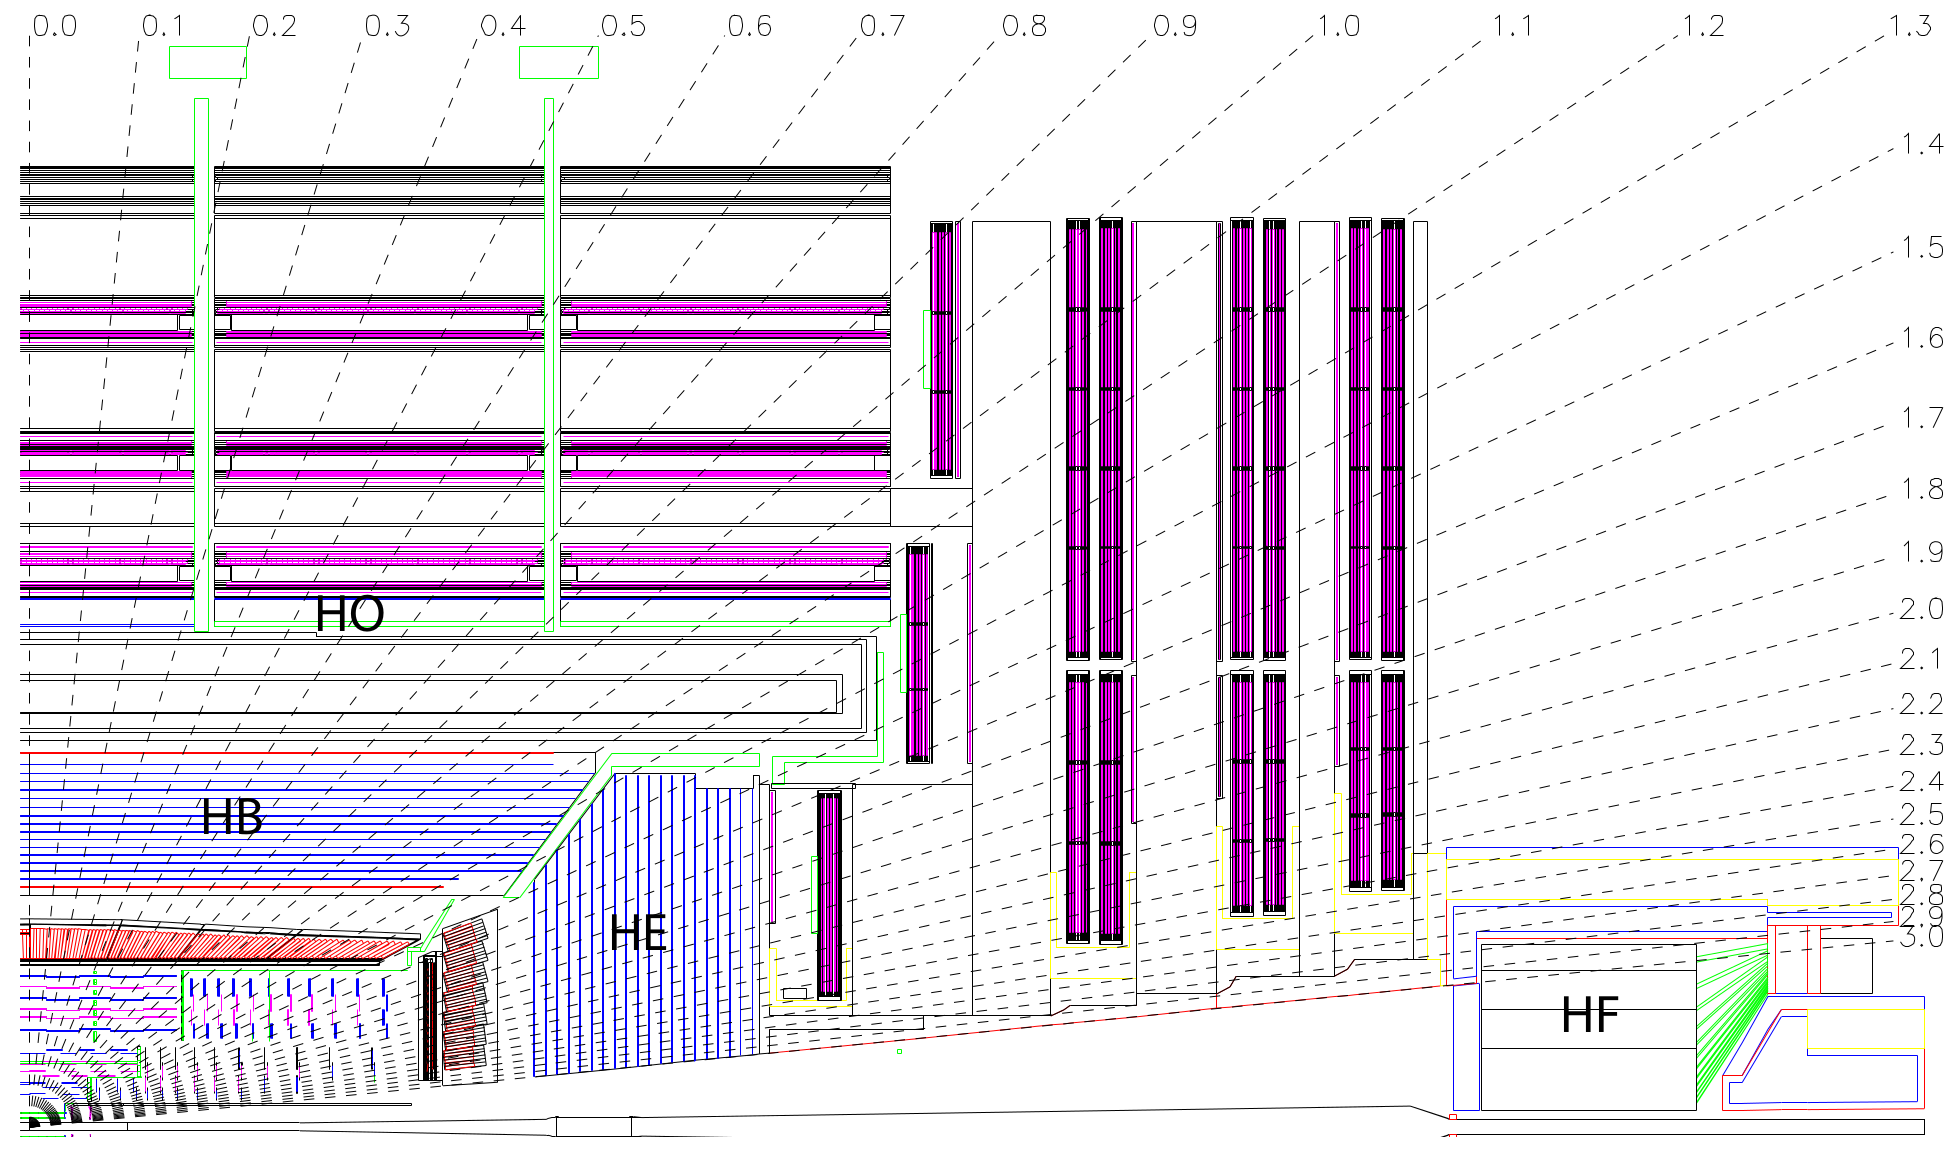
\includegraphics[width=0.8\textwidth]{\PhDthesisdir/plots_and_images/from_cms_paper/fig_5-1.png}
\caption[Schéma du calorimètre hadronique de CMS.]{Schéma d'un cadrant du détecteur CMS~\cite{cms_paper} montrant la localisation des calorimètres hadroniques du \CMSbarrel\ (HB), externe (HO), du \CMSendcap\ (HE) et \CMSforward\ (HF). Certaines valeurs de $\eta$ et les directions associées sont indiquées.}
\label{fig-chapter-LHC-section-CMS-subsec-HCAL-cms_paper-fig_5-1}
\end{figure}
\par Tout comme le ECAL, il comporte un \CMSbarrel\ (HB) couvrant la région $\abs{\eta}<\num{1.3}$ et deux \CMSendcaps\ (HE) couvrant $\num{1.3}<\abs{\eta}<\num{3}$.
Le HCAL est composé de couches alternées d'absorbeurs et de scintillateurs.
L'absorbeur, du laiton, permet d'initier la gerbe hadronique.
%Les muons interagissant peu avec ce matériau, leur mesure par les chambres à muons situées au-delà du HCAL est donc peu perturbée par leur traversée du HCAL.
Le scintillateur est fait en plastique.
Des fibres optiques permettent de recueillir la lumière émise par les gerbes hadroniques.
La mesure de ce signal lumineux donne une mesure de l'énergie des hadrons.
\par Cependant, le nombre de longueurs d'interaction combinées des ECAL et HCAL dans le \CMSbarrel, de l'ordre de dix, est insuffisant pour contenir toutes les gerbes hadroniques~\cite{cms_paper}.
Le HB est ainsi complété par un calorimètre hadronique externe (HO) installé sur la face interne de la culasse, \ie\ de l'autre côté du solénoïde et avant les chambres à muons.
\begin{wrapfigure}{R}{.5\textwidth}
\centering
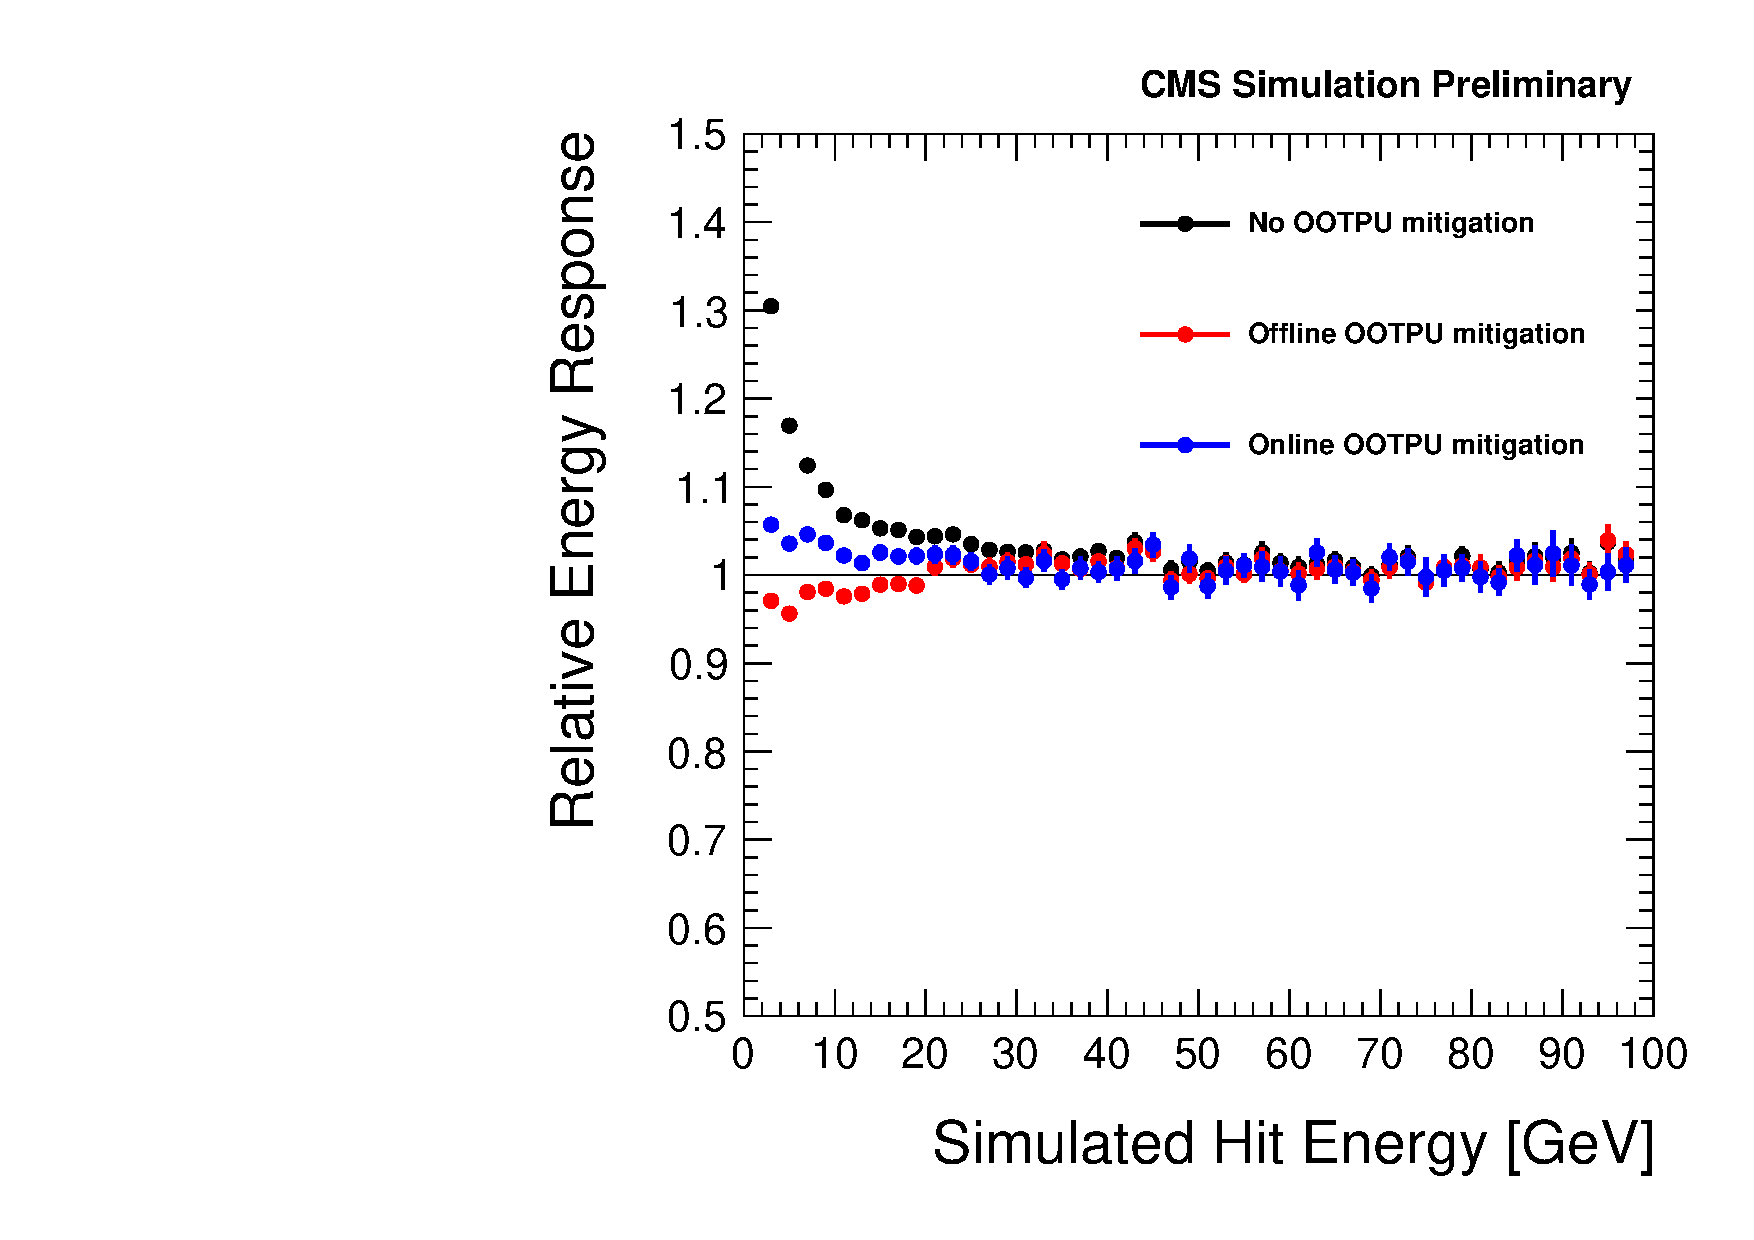
\includegraphics[width=0.45\textwidth]{\PhDthesisdir/plots_and_images/from_CMS-DP-2016-071/hcal_method2_3_performance.pdf}
\caption[Réponse relative du calorimètre hadronique de CMS.]{Réponse relative du calorimètre hadronique de CMS~\cite{CMS-DP-2016-071} en fonction de l'énergie simulée du dépôt, estimée par simulation. En noir, sans correction de l'empilement asynchrone (OOTPU). En bleu, avec des corrections en ligne, \ie\ un ajustement des amplitudes et temps d'arrivée des signaux en prenant en compte jusqu'à trois signaux avant et après le signal d'intérêt. En rouge, avec l'ensemble des corrections.}
\label{fig-chapter-LHC-section-CMS-subsec-HCAL-CMS-DP-2016-071-hcal_method2_3_performance}
\end{wrapfigure}
\par Enfin, une couverture plus large en $\eta$ est assurée par le calorimètre hadronique \CMSforward\ (HF) couvrant $\num{2.9}<\abs{\eta}<\num{5.2}$.
Les deux HF, un à chaque extrémité de CMS, sont des détecteurs cylindriques ayant des absorbeurs en acier dans lesquels passent des fibres optiques de quartz.
Les particules incidentes émettent de la lumière Cherenkov lors de leur passage, cette lumière est alors recueillie par les fibres optiques.
\par La réponse relative du HCAL, \ie\ l'énergie reconstruite dans le HCAL par rapport à l'énergie effective du dépôt a été estimée par simulation et est représentée en fonction de l'énergie simulée du dépôt sur la figure~\ref{fig-chapter-LHC-section-CMS-subsec-HCAL-CMS-DP-2016-071-hcal_method2_3_performance}.
Elle ne dévie pas de plus de \SI{5}{\%} au-delà de \SI{10}{\GeV}~\cite{CMS-DP-2016-071} une fois que l'empilement asynchrone, défini dans la section~\ref{chapter-LHC-section-LHC-subsec-PU}, est retiré~\cite{CMS-DP-2016-071,CMS-DP-2018-018}.
Comme dans le cas du ECAL, la réponse du HCAL évolue au cours du temps~\cite{CMS-DP-2017-033} et doit être contrôlée.
La résolution $\sigma$ obtenue sur l'énergie des hadrons, par combinaison avec les signaux du ECAL, a été déterminée à l'aide d'un faisceau test de pions comme étant
\begin{equation}
\frac{\sigma}{E} = \frac{\num{1.1}}{\sqrt{E}} + \num{0.09}
\end{equation}
où $E$ est l'énergie mesurée en \SI{}{\GeV}.